\documentclass
   [kulak] % options: kul/kulak, handout (altijd kul of kulak optioneel kan handout bijgevoegd worden)
   {kulakbeamer}

\usepackage[dutch]{babel}
\usepackage[utf8]{inputenc}
\usepackage[T1]{fontenc}
\usepackage{listings}
\usepackage{color}
\usepackage{graphicx}

\lstset{
	mathescape
}

\lstdefinestyle{CStyle}{
	breakatwhitespace=false,         
	breaklines=true,                 
	captionpos=b,                    
	keepspaces=true,                 
	numbers=left,                    
	numbersep=5pt,                  
	showspaces=false,                
	showstringspaces=false,
	showtabs=false,                  
	tabsize=2,
	language=C,
	morekeywords={parallel, spawn, sync, new}
}




\title[Multithreaded Algorithms]{Multithreaded Algorithms}
\author[T. Bamelis]{Thomas Bamelis} 
\institute[Kulak]{KU Leuven Kulak}
\date{Academiejaar 2017-2018}

\defbeamertemplate{description item}{align left}{\insertdescriptionitem\hfill}

% Overzicht bij het begin van elk hoofdstuk 
\AtBeginSection[]{\only<beamer>{\addtocounter{framenumber}{-1}
	\begin{outlineframe}[Overzicht]
		\tableofcontents[currentsection]
	\end{outlineframe}}
	}

\begin{document}

\begin{titleframe}
\titlepage
\end{titleframe}

\begin{outlineframe}[Overzicht]
\tableofcontents
\end{outlineframe}

 % % % Here you go  % % % 

\section{Inleiding}

\begin{frame}
\frametitle{Multiprocessoren en threads}

\setbeamertemplate{description item}[align left]
\begin{description}[Other description]
	\pause
	\item[\textbf{Multiprocessors}]
	\pause 
	\begin{itemize}
		\item  Meerder processors en/of cores per processor
		
		\item  Meerdere instructies simultaan
	\end{itemize}
	
	\itemsep=2em
	\pause
	
	\item[\textbf{Threading}] 
	
	
	\pause
	
	
	\begin{itemize}
		\item  Apart (parallel) uitgevoerd
		
		\item Heeft : ID, PC, registers en stack
		
		\item Deelt : code- en data sections en resources (e.g. file)
		
	\end{itemize}  
\end{description}

\end{frame}

\begin{frame}
	\frametitle{Dynamic threading}
	
	Toegankelijke vorm van threading met enorm potentieel.\\
	Scheduler beslist hoeveel threads wanneer.\\ IPV thread maken, thread suggereren.
	
	 
	
	\begin{description}[align=parleft]
		
		\item[\textbf{Nested parallalism}]
		
		Een thread kan andere threads oproepen
		
		\itemsep=2em
		\item[\textbf{Parallel loop}]
		
		Iedere iteratie in een for loop voert tegelijk uit
		
	\end{description}
	
	
\end{frame}

\section[Basis]{Basis van multithreading}


\begin{frame}[fragile]
	\frametitle{Voorbeeld}
	
	Voorbeeld m.b.v. (slechte) recursieve Fibonacci $= \Theta(\phi^n)$ \\ met
	$\phi = (1 + \sqrt{5})/2$ de `gouden ratio'
	
	
	
	\begin{columns}[T] % align columns
		
		
		
		\begin{column}{.48\textwidth}
			\begin{minipage}[c][.6\textheight][c]{\linewidth}
				F\textsubscript{0} = 0 \\
				F\textsubscript{1} = 1 \\
				F\textsubscript{i} = F\textsubscript{i-1} + F\textsubscript{i-2} als i $\geqslant$ 2  
				
				
				
				
				
			\end{minipage}
		\end{column}
		
		
		
		\begin{column}{.48\textwidth}
	
	Fib(n)
	\begin{lstlisting}[style=CStyle]
	
	if n <= 1
		return n
	else 
		x = Fib(n-1)
		y = Fib(n-2)
		return x + y
	
	\end{lstlisting}
	
	\end{column}
	
	
	
	

	\end{columns}
	
\end{frame}



\begin{frame}
	\frametitle{Keywords}
	
	\begin{description}
		\pause
		
		
		\item[\textbf{spawn}] Geeft aan dat de subroutine parallel kan worden uitgevoerd. Nested-parallism mogelijk (child kan andere threads oproepen).
		
		\pause
		\itemsep=2em
		\item[\textbf{sync}] Wachten tot alle children voltooien (impliciet in iedere return)
		
		
		
		
		
	\end{description}
	
	
\end{frame}




\begin{frame}[fragile]
	\frametitle{Parallel voorbeeld}
	
	
	
	\begin{columns}[T] % align columns
		\begin{column}{.48\textwidth}
			\begin{minipage}[c][.6\textheight][c]{\linewidth}
				
				
				
				
				
				
				\begin{description}
					\item[\textbf{`Logical parallelism'}] subroutine \textit{kan} parallel uitvoeren
					\itemsep=2em
					\item[\textbf{Serialization}] Threading keywoorden weglaten geeft sequentieel algoritme
				\end{description}
				
			\end{minipage}
		\end{column}
	


\begin{column}{.48\textwidth}

P-Fib(n)
\begin{lstlisting}[style=CStyle]

if n <= 1
	return n
else 
	x = spawn P-Fib(n-1)
	y = P-Fib(n-2)
	sync
	return x + y

\end{lstlisting}

\end{column}

\end{columns}

\end{frame}




\begin{frame}
	\frametitle{Voorstelling multithreaded algoritme}
	\pause
	Gerichte kringloze graaf G(V,E) \\ (`Computation dag')
	
	\begin{itemize}
		\item V de verzameling instructies (of strands)
		
		\item E met  (u,v) $\in$ E: \textit{ u moet voor v uitvoeren.}
		\item[]
		
	\end{itemize}
	
	\begin{description}
		
	
	\pause \item
	[\textit{Strand}] stuk zonder parallelle keywords \\
	\pause \itemsep=1em \item
	[Strands $u$ en $v$ \textit{`in serie'}] indien direct pad (u,v) $\in$ E, \\ anders \textit{in parallel}
\end{description}
\end{frame}


\begin{frame}
	\frametitle{Soorten bogen}
	\pause
	\begin{description}[align=parleft]
		\item[\textbf{Continuation boog $(u,u')$}]
		Strand $u$ die (in dezelfde thread) direct doorgaat naar volgende strand $u'$
		\pause
		\item[\textbf{Spawn boog $(u,v)$}]
		Strand $u$ `spawnt' strand $v$ (mogelijks in andere thread)
		\pause
		\item[\textbf{Call boog $(u,v)$}]
		Strand $u$ doet functieoproep naar functie $v$ (in zelfde thread)
		\pause
		\item[\textbf{Return boog $(u,x)$}]
		Gespawnde strand $u$ keert terug naar parentprocedure met $x$ de eerste strand na de eerstvolgende sync na spawn $u$
	\end{description}
	
	\pause
	
	Iedere strand $u$ die strand $v$ spawnt, heeft ook cont. boog $(u,u')$ 
\end{frame}


\begin{frame}
\frametitle{P-Fib(4)}


	\begin{columns}[T]
		\begin{column}{.7\textwidth}
		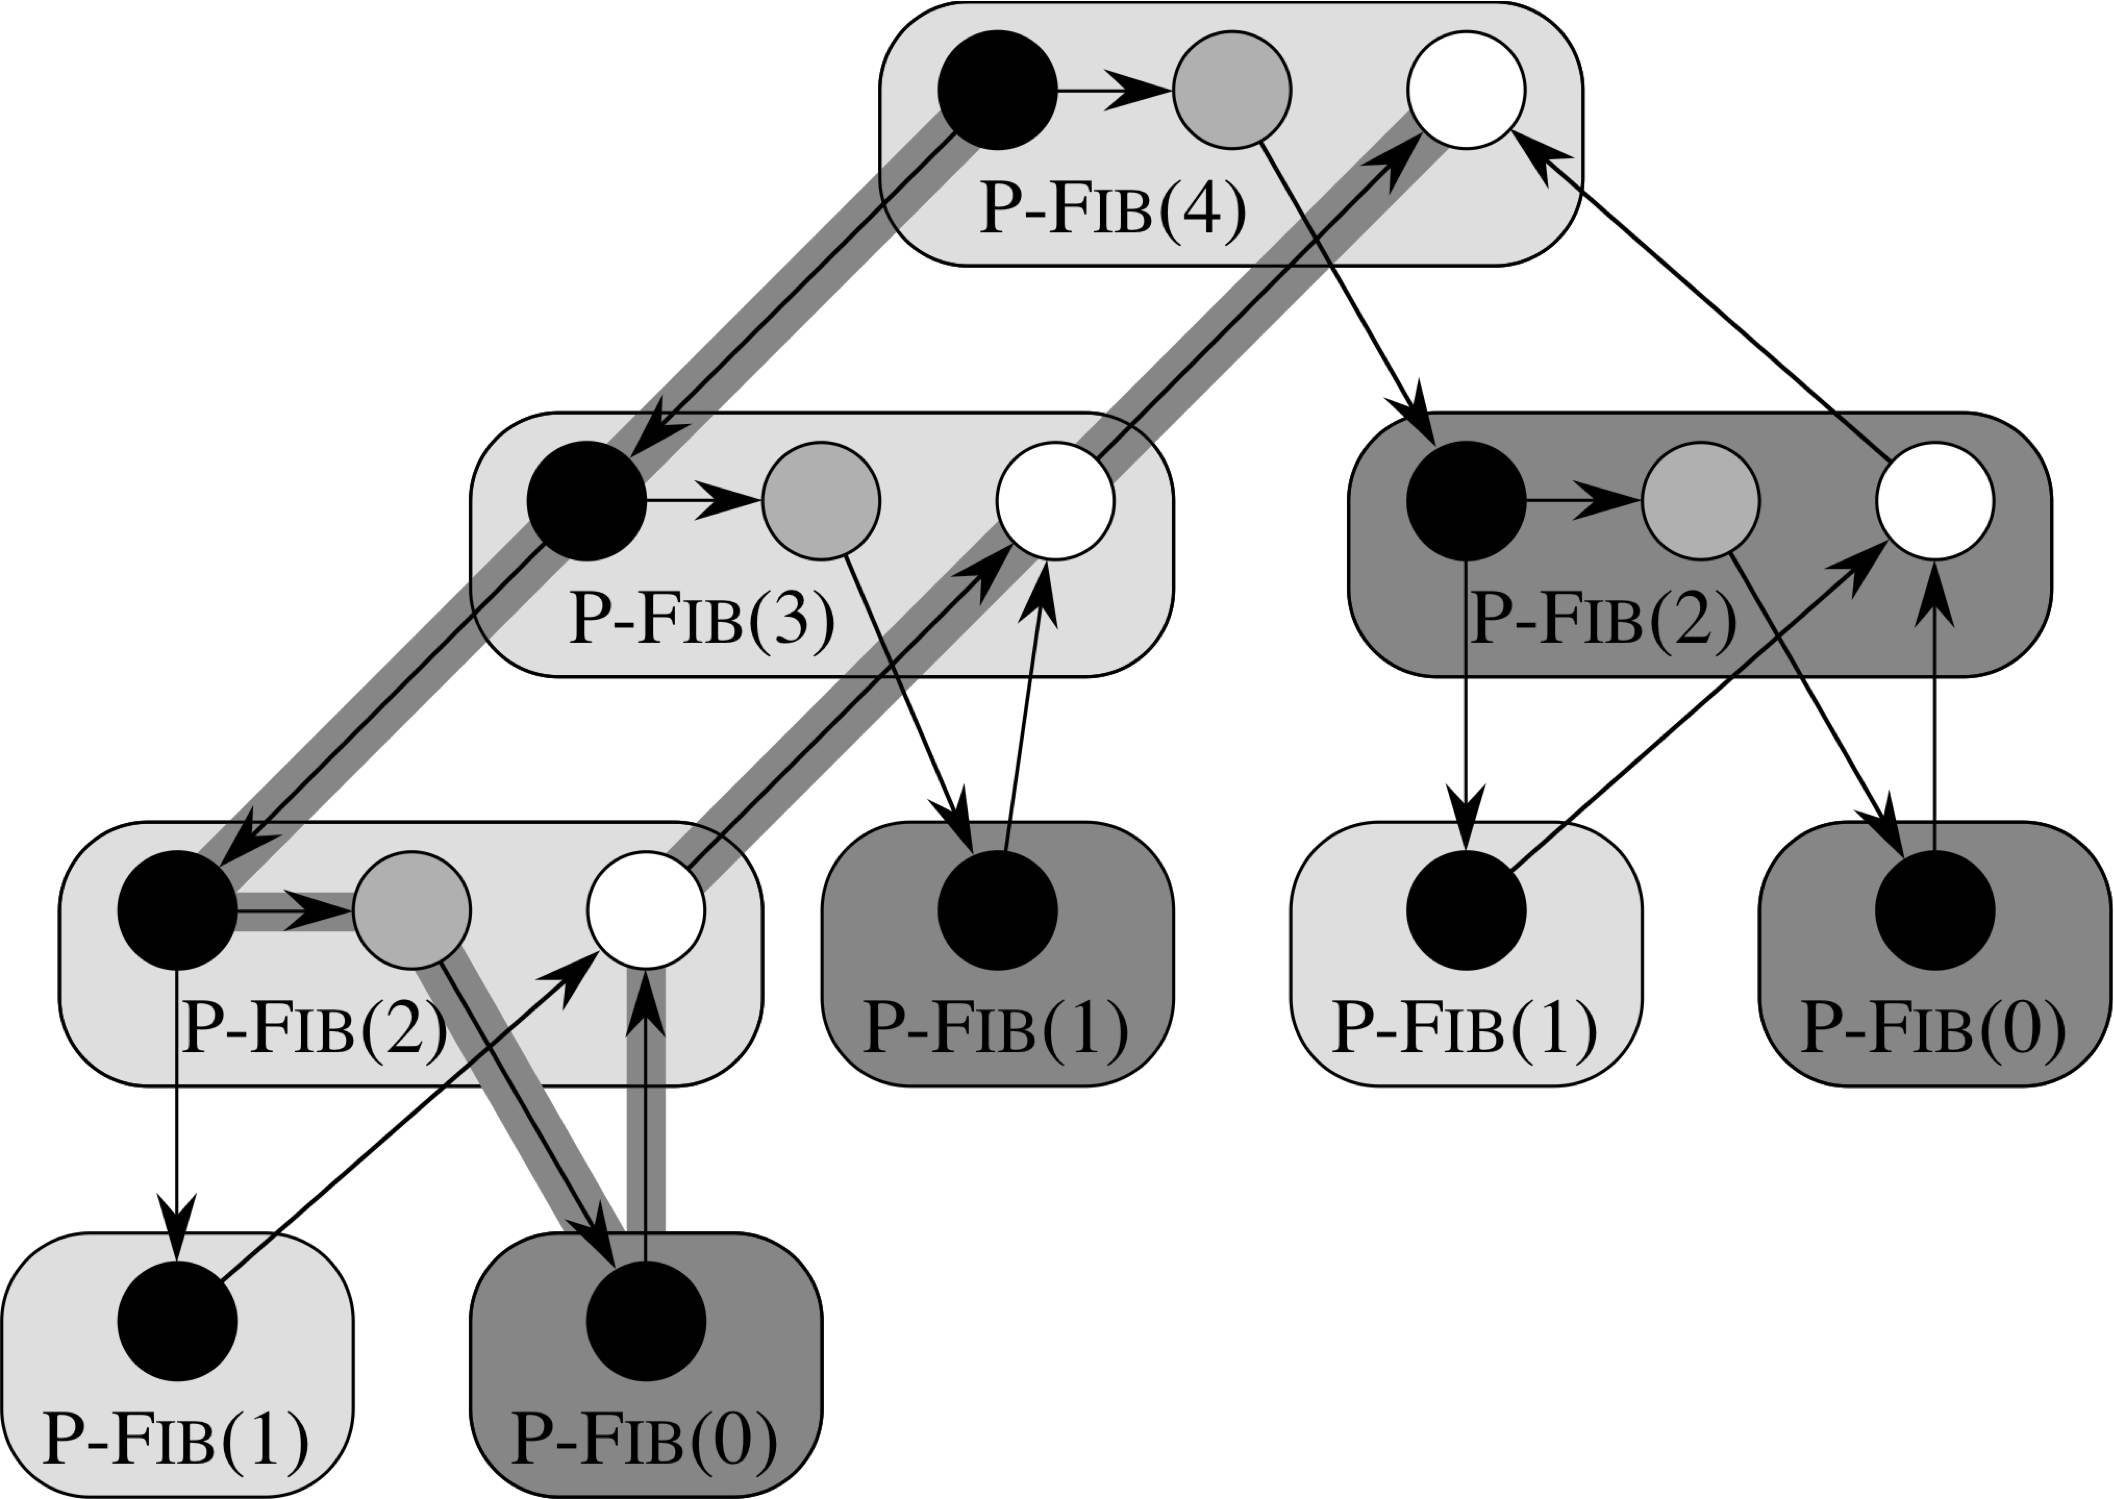
\includegraphics[height=0.7\textheight]{fig2.jpg}			
		\end{column}
	\begin{column}{.25\textwidth}
		\begin{minipage}[c][.6\textheight][c]{\linewidth}
			
			\begin{itemize}
				\item Bol: strand
				\item Hor. pijl: cont. boog
				\item Ver./Dig. pijl (neerwaarts): spawn of call boog
				\item Ver./Dig. pijl (opwaarts): return boog
				
			\end{itemize}
			
		\end{minipage}
	\end{column}
	\end{columns}
	
\end{frame}


\begin{frame}[fragile]
	\frametitle{Strands in P-Fib}
	Bu / Eu : Begin strand u / End strand u
	\begin{columns}[T]
		\begin{column}{.8\textwidth}
			
		
	
	
	\begin{lstlisting}[style=CStyle]
	P-Fib(n) 
	/*Bu*/
	if n <= 1
	return n
	else 
	x = /*Eu*/ spawn /*Bv*/ P-Fib(n-1) /*Ev*/
	/*Bu'*/
	y = /*Eu'*/ /*Bv'*/ P-Fib(n-2)
	/*Ev'*/
	sync
	return /*Bx*/ x + y /*Ex*/\end{lstlisting}
	
\end{column}

\begin{column}{.2\textwidth}
	\pause
	\textbf{Bogen\\ $(i \leqslant 2)$:}
	\\ \pause
	-Spawn $(u,v)$
	\\ \pause
	-Cont $(u,u')$
	\\ \pause
	-Call $(u',v')$
	\\ \pause
	-Return $(v,x)$ $(v',x)$
	
	
	\pause
	
	$\ast$  sync in return --> Parallel keyword
\end{column}

\end{columns}
	
\end{frame}



\begin{frame}
	\frametitle{Ideale parallelle computer}
	\pause
	\begin{itemize}
		
		\item Iedere processor even vlug
		
		\pause
		
		\item Sequentially consistent: Alsof 1 instructie-cyclus van alle processoren maar 1 geheugentoegang nodig was
		
		\pause
		
		\item Geen scheduling kost (in realiteit minimaal)
	\end{itemize}
	
\end{frame}

\section[Meeteenheden]{Meeteenheden prestatie}

\begin{frame}
	\frametitle{Prestatie meten}
	
	Hoe kwaliteit meten van een algoritme? \\~\\~\\
	\pause
	\begin{columns}[T]
		\begin{column}{.45\textwidth}
			\textbf{\textit{work}}
			\begin{itemize}
				\item Tijd om op 1 processor uit te voeren
				\itemsep=2em
				\item[$\ast$] \textit{bij 1 tijdseenheid per strand, aantal knopen}
			\end{itemize}
		\end{column}
		\begin{column}{.45\textwidth}
			\pause
			\textbf{\textit{span}}
			\begin{itemize}
				\item De tijd van het meest tijdsintensieve pad
				\itemsep=2em
				\item[$\ast$] \textit{bij 1 tijdseenheid per strand, lengte langste (critical) pad}
			\end{itemize}
		\end{column}
	\end{columns}
	\pause
	~\\~\\
	\textit{T\textsubscript{P} = tijd op P processors}\\
	work = T\textsubscript{1} en span = T\textsubscript{$\infty$}
\end{frame}

\begin{frame}
	\frametitle{Span}
	
	\begin{columns}[T]
		\begin{column}{.7\textwidth}
			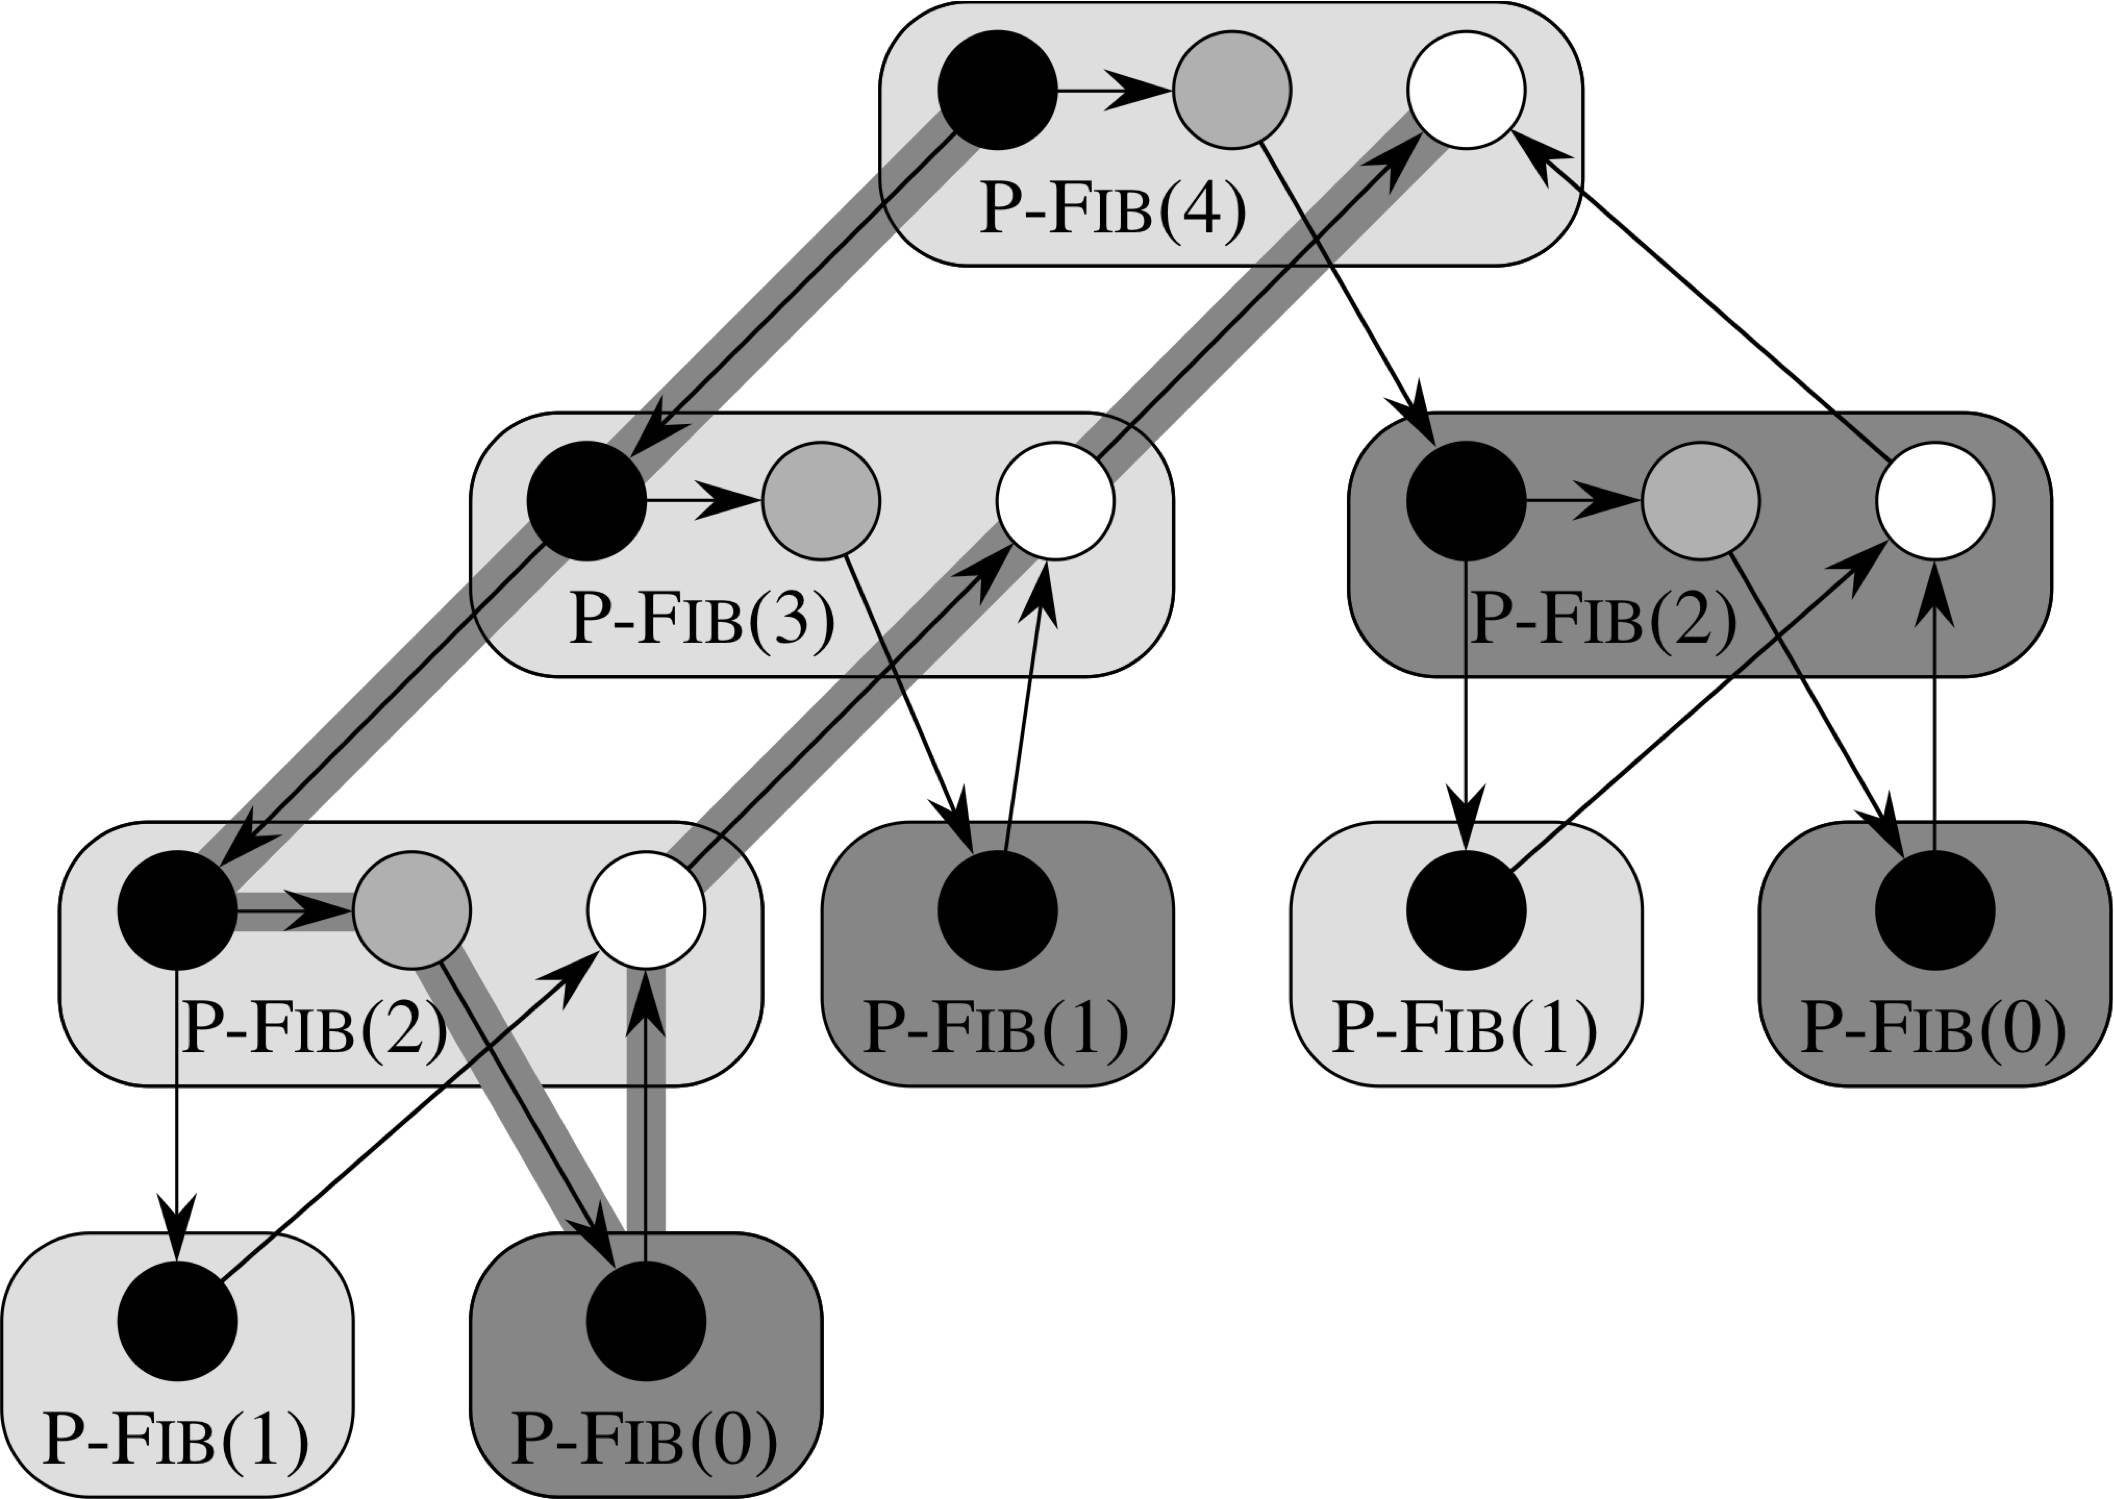
\includegraphics[height=0.7\textheight]{fig2.jpg}			
		\end{column}
		\begin{column}{.25\textwidth}
			\begin{minipage}[c][.6\textheight][c]{\linewidth}
				\begin{itemize}
					\item[]Span is de dikke lijn.
				\end{itemize}
				
				
			\end{minipage}
		\end{column}
	\end{columns}
\end{frame}

\begin{frame}
	\frametitle{Ondergrenzen}
	Work en span zorgen voor ondergrenzen. \\~\\
	
	\pause
	
	\textit{work law}
	\begin{itemize}
		\item[$\bullet$] $T\textsubscript{P} \geqslant T\textsubscript{1}/P$
		\begin{itemize}
			\item[] P processoren $\Rightarrow$ P werkeenheden / tijdseenheid\\ $\Rightarrow$ $PT\textsubscript{P}$ werkeenheden in T\textsubscript{P} tijd\\EN\\ Totaal werk = work $\Rightarrow$ $PT\textsubscript{P} \geqslant T\textsubscript{1}$
		\end{itemize}
	\end{itemize}
	  
	\pause
	  
	\textit{span law}
	\begin{itemize}
		\item[$\bullet$] $T\textsubscript{P} \geqslant T$\textsubscript{$\infty$} 
		
		\begin{itemize}
			\item[] P processoren systeem altijd trager of even vlug als $\infty$ processoren. \textit{($\infty$ kan P na-apen)}
		\end{itemize}
	\end{itemize}
	
\end{frame}


\begin{frame}
	\frametitle{Speedup}
	$\rightarrow$ \textbf{\textit{Speedup}}: hoeveel sneller met P processoren dan 1 uitgedrukt met:
	$T\textsubscript{1}/T\textsubscript{P}$
	\pause
	\\
	Met bovengrens P (work law)\\~\\
	\pause
	\begin{description}
		\item[\textbf{Linear speedup}]
		 $ T\textsubscript{1}/T\textsubscript{P} = \Theta(P) $
		\itemsep=2em
		\pause
		\item[\textbf{Perfect linear speedup}] $ T\textsubscript{1}/T\textsubscript{P} = P $
	\end{description} 
	
\end{frame}

\begin{frame}
	\frametitle{Parallelism}
	$\rightarrow$ \textbf{\textit{Parallelism}}: hoeveel voordeel door multi-threading uitgedrukt met: $T\textsubscript{1}/T$\textsubscript{$\infty$} \\~\\
	\pause
	3 interpretaties:
	\begin{enumerate}
		\item \textit{Ratio}: gemiddeld werk per stap in langste pad vergeleken met gemiddelde werk per stap van $T_1$ ( = work en langste pad = span)
		
		\pause
		\item \textit{Bovengrens}: maximum speedup
		
		\pause
		\item \textit{Mogelijkheid perfect lineair}: Indien \# processoren Q groter is dan parallellisme, geen perfecte lineariteit mogelijk. (want $T_Q \geqslant T_\infty$)
	\end{enumerate}
\end{frame}

\begin{frame}
\frametitle{Vb parallellisme}

\begin{columns}[T]
	\begin{column}{.6\textwidth}
		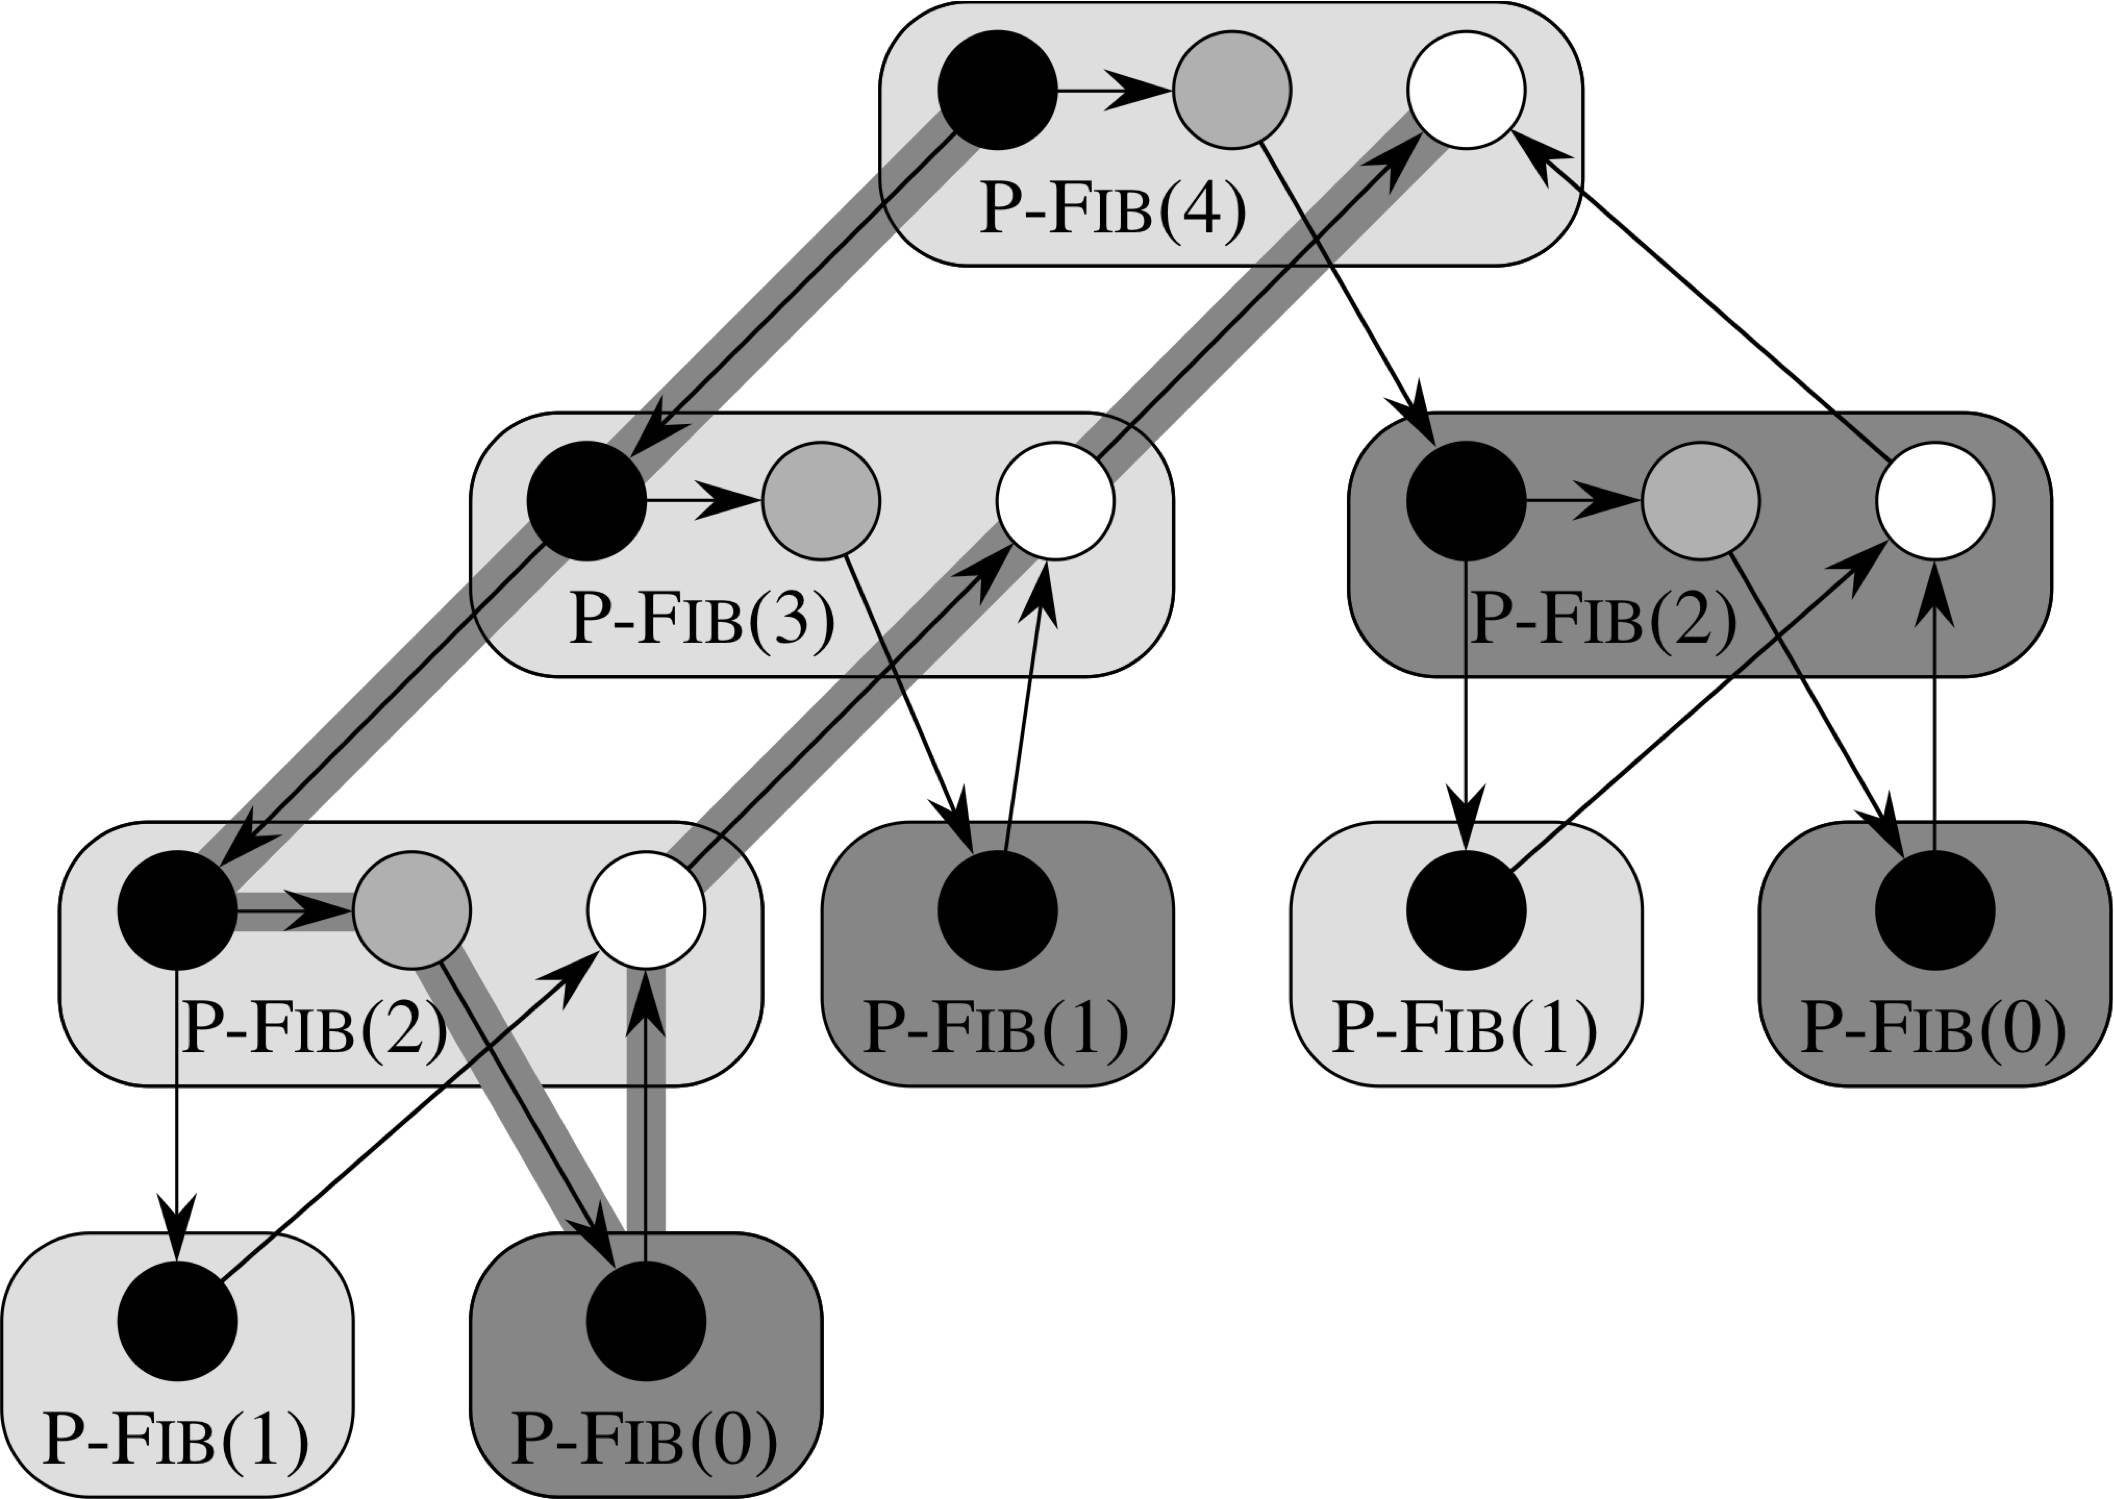
\includegraphics[width=\textwidth]{fig2.jpg}			
	\end{column}
	\begin{column}{.35\textwidth}
		\begin{minipage}[c][.6\textheight][c]{\linewidth}
			\begin{itemize}
				\item[] work = T\textsubscript{1} = 17
				\item[] span = T\textsubscript{$\infty$} = 8 (dikke lijn)
				\item[] parallelism = T\textsubscript{1}/T\textsubscript{$\infty$} = 2,125
				\item[$\rightarrow$] max 2,125 sneller
				
			\end{itemize}
			
			
		\end{minipage}
	\end{column}
\end{columns}
\end{frame}

\begin{frame}
	\frametitle{Slackness}
	Verhouding tussen parallellisme algoritme en computer met P processors\\~\\
	$\frac{parallellisme}{P} = \frac{T\textsubscript{1}/T_\infty}{P} =  \frac{T\textsubscript{1}}{PT_\infty}$ ~\\~\\
	\textit{`Hoeveel meer/minder parallellisme dan processors'}\\~\\
	Onder 1 $\rightarrow$ meer processors dan parallellisme $\rightarrow$ niet perfect lineair \\~\\
	Boven 1 $\rightarrow$ minder processors dan parallellisme $\rightarrow$ mogelijks perfect lineair \\ $\Rightarrow$Processors zijn hierbij de limiterende factor
\end{frame}

\section[Scheduling]{Scheduling van threads}

\begin{frame}
\frametitle{Scheduling}
\begin{description}
\item
 [Algemeen]: Een scheduler beslist of er een thread aangemaakt wordt bij een spawn en mapped op static string.\\Beslissing hangt af van momentele belasting computer.\\~\\ 
\end{description}
$\triangleright$ Waarom? \\~\\ Strands efficiënt parallel uitvoeren:\\
$\rightarrow$ te veel zorgt voor trashing \\
$\rightarrow$ te weinig voor onderbenutting
\end{frame}

\begin{frame}
	\frametitle{Kenmerken beschouwde scheduler}
	\begin{description}
		\item[\textbf{Centralized}] De scheduler weet op ieder moment de load van de computer.
		\item[\textbf{Greedy}] De scheduler creëert zoveel mogelijk threads bij iedere stap.
		\item[Complete stap] Er zijn P strands klaar om uit te voeren op ieder tijds stap. Minder is incomplete.
	\end{description}
\end{frame}

\begin{frame}
	\frametitle{Perfomance greedy schedular}
	\textbf{Stelling 27.1}\\
	Gegeven een ideale parallelle computer met $P$ processors, een greedy scheduler en een algoritme met span = $T_\infty$ en work = $T_1$\\
	$\Rightarrow T_P \leqslant \frac{T_1}{P} + T_\infty$ \\~\\~\\
	Bovengrens work law = $T_P \leqslant \frac{T_1}{P}$ en span law $T_P \leqslant T_\infty$ \\
	$\rightarrow$ Niet slecht.
\end{frame}

\begin{frame}
	\frametitle{Bewijs stelling 27.1}
	\begin{itemize}
		\item [1)] \textbf{Complete stap}\\
		P processors $\Rightarrow P \frac{werk}{stap}$ \\
		Stel aantal complete stappen $> \lfloor T_1/P\rfloor$
		\pause \\
		$\Rightarrow$ dan is het total werk minstens
		
		
		\begin{equation} 
		\begin{split}
		P\cdot (\lfloor T_1 /P\rfloor + 1) & = P\cdot\lfloor T_1 /P\rfloor + P  \\
		& = T_1 - (T_1 \mod P) + P \\
		& > T_1  
		\end{split}
		\end{equation}
		
		*\textit{want: $a\mod n = a - n\lfloor a/n\rfloor$}\\
		**\textit{want:  $0 \leqslant a\mod n < n$} \\ ~ \\
		\pause
		\textbf{\textit{CONTRADICTIE:}} meer werk dan $T_1$\\$ \Rightarrow$ aantal complete stappen $\leqslant \lfloor T_1 /P\rfloor$ \\
		
	\end{itemize}
\end{frame}

\begin{frame}
	\frametitle{Bewijs stelling 27.1}
	\begin{itemize}
		\item[2)] \textbf{Incomplete stap}\\ 
		Stel graaf G de graaf die het algoritme voorstelt:
		\\ Maak alle bogen gewicht 1 door langere bogen op te splitsen.\\
		\pause
		$\rightarrow$ G' subgraaf uit te voeren voor de incomplete stap  \\
		$\rightarrow$ G'' uit te voeren erna\\
		$\rightarrow$ Startknoop cruciaal pad geen inkomende bogen = uitvoerbaar (anders niet start)\\
		\pause
		$\Rightarrow$ Incomplete stap voert alle zulke bogen uit in G' \\(want minder dan P strands en greedy ) \\
		$\Rightarrow$ Lengte cruciale pad G'' 1 korter dan van G'\\
		$\Rightarrow$ Span = Span - 1 na stap\\
		$\Rightarrow$ Aantal incomplete stappen $\leqslant$ span $= T_\infty$
	\end{itemize}
\end{frame}

\begin{frame}
	\frametitle{Bewijs stelling 27.1}
	
	$T_P =$ \# complete + \# incomplete stappen $= \lfloor T_1 /P\rfloor + T_\infty$ \\~\\
	$\Rightarrow T_P \leqslant \lfloor T_1 /P\rfloor + T_\infty$\\
	\flushright{$\Box$}
	
\end{frame}

\begin{frame}
	\frametitle{Gevolg 27.2}
	Stel zelfde aannames stelling 27.1, dan is $T_P$ maximum 2 keer de optimale tijd. \pause \\~\\
	\textbf{Bewijs}\\
	Stel $T_P^*$ optimale tijd\\
	$\Rightarrow T_P  \leqslant \frac{T_1}{P} + T_\infty \leqslant 2\cdot\max(\frac{T_1}{P} , T_\infty)$ (27.1)
	\[
		\begin{cases}
		 T_P  \leqslant 2\cdot\max(\frac{T_1}{P} , T_\infty) & \\
		 T_P^* \geqslant \max(\frac{T_1}{P} , T_\infty) & \text{work en span law}
		\end{cases}
	\]
	$\Rightarrow T_P \leqslant 2T_P^*$
	\flushright{$\Box$}
\end{frame}

\begin{frame}
	\frametitle{Gevolg 27.3}
	Stel zelfde aannames stelling 27.1 .
	\\ Als $P << \frac{T_1}{T_\infty} =$ slackness, dan $T_P \approx \frac{T_1}{P} $ \\
	Dus de speedup $\approx P$ en dus bijna perfect lineair.\\ $<< \approx$ 10 keer zo groot, dan is $T_\infty$ in $T_P \leqslant \frac{T_1}{P} + T_\infty$ kleiner dan 10\% van $\frac{werk}{processor}$  \pause \\~\\
	\textbf{Bewijs} ~~~~~~~
	Stel $P << \frac{T_1}{T_\infty}$ \\
	$\Rightarrow T_\infty << \frac{T_1}{P} $ \\
	$\Rightarrow \frac{T_1}{P} + T_\infty \approx \frac{T_1}{P} $ \\
	\[
		\begin{cases}
			\frac{T_1}{P} + T_\infty \approx \frac{T_1}{P} & \\
			T_P \leqslant \frac{T_1}{P} + T_\infty & \text{(27.1)}  \\
			T_P \geqslant \frac{T_1}{P} & \text{work law}
		\end{cases}
	\]
	$\Rightarrow T_P \approx \frac{T_1}{P} \Rightarrow \frac{T_1}{T_P}\approx P$ ~~~~~~~~~~~~~~~~~~~~~~~~~~~~ $\Box$
	
\end{frame}

\section[Analyse]{Analyseren van een algoritme}

\begin{frame}
	\frametitle{Analyseren van een algoritme}
	\begin{enumerate}
		\item \textbf{\textit{Work}}: Hetzelfde zoals seriële algoritmen.
		\pause
		\itemsep=3em
		\item \textbf{\textit{Span}}: Wordt nu besproken.
	\end{enumerate}
\end{frame}

\begin{frame}[fragile]
	\frametitle{Vb met P-Fib}
	P-Fib(n)
	\begin{lstlisting}[style=CStyle]
	if n <= 1
	return n
	else 
	x = spawn P-Fib(n-1)
	y = P-Fib(n-2)
	sync
	return x + y
	\end{lstlisting}
	
	~\\In serie: $T(n) = T(n-1) + T(n-2) + \Theta(1)$ \\~\\
	Work = $T_1 (n) = \Theta(\phi^n)$ uit vorige\\ met
	$\phi = (1 + \sqrt{5})/2$ de `gouden ratio'
	
\end{frame}

\begin{frame}
	\frametitle{Vb met P-Fib}
	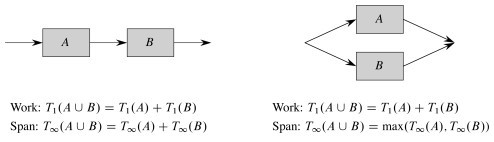
\includegraphics[width=\textwidth]{fig3.jpg}
	\\Span: als 2 strands in serie staan worden ze opgeteld. \\ In parallel wordt het maximum opgeteld bij de span. \pause \\
	$\rightarrow T_\infty (n) = \max(T_\infty (n-1),T_\infty (n-2)) + \Theta(1)$\\
	$\rightarrow T_\infty (n) = T_\infty (n-1) + \Theta(1)$ \\
	$\rightarrow T_\infty (n) = \Theta(n)$\\~\\
	\pause 
	Parallellisme $= \frac{T_1 (n)}{T_\infty (n)} = \Theta(\frac{\phi^n}{n})$ wordt zeer groot als n groeit \\$\rightarrow$ al snel baat bij veel processors als n groeit
	
\end{frame}


\begin{frame}[fragile]
\frametitle{Parallel loops}

Loops waarvan de iteraties parallel kunnen uitvoeren. \\ \textit{Keyword}: parallel for\\
\textit{Keyword}: new j = iedere iteratie eigen versie variabele j

\pause

\begin{columns}[T] % align columns
	
	
	
	\begin{column}{.3\textwidth}
		\begin{minipage}[c][.6\textheight][c]{\linewidth}
				
			\textbf{VB: nxn matrix A $\cdot$ n-vector X}
			\\
			\[
			y_i = \sum_{j=1}^n a_{ij}x_{j}
			\]
			
		\end{minipage}
	\end{column}
	
	
	
	\begin{column}{.65\textwidth}
		
		Mat-Vec(A,X)
		\begin{lstlisting}[style=CStyle]
		
		n = A.rows
		init y als n-vector
		parallel for i = 1 to n
			for new j = 1 to n
				$y_i = y_i + a_{ij}x_{j}$
		return y
		\end{lstlisting}
		
	\end{column}
	
	
	
	
	
\end{columns}

\end{frame}

\begin{frame}[fragile]
	\frametitle{Parallel loops}
	
	Work = $\Theta$ serie = $\Theta(n^2)$ (overhead scheduler groeit niet asymptotisch mee)
	
	\begin{columns}[T] % align columns
		
		
		
		\begin{column}{.3\textwidth}
			\begin{minipage}[c][.6\textheight][c]{\linewidth}
				
				\textbf{VB: nxn matrix A $\cdot$ n-vector X}
				\\
				\[
				y_i = \sum_{j=1}^n a_{ij}x_{j}
				\]
				
			\end{minipage}
		\end{column}
		
		
		
		\begin{column}{.65\textwidth}
			
			Mat-Vec(A,X)
			\begin{lstlisting}[style=CStyle]
			
			n = A.rows
			init y als n-vector
			parallel for i = 1 to n
				for new j = 1 to n
					$y_i = y_i + a_{ij}x_{j}$
			return y
			\end{lstlisting}
			
		\end{column}

	
		
	\end{columns}
	
\end{frame}

\begin{frame}[fragile]
	\frametitle{Parallel loop span}
	
	Loops waarvan de iteraties parallel kunnen uitvoeren. \\ \textit{Keyword}: parallel for\\
	\textit{Keyword}: new j = iedere iteratie eigen versie variabele j
	
	
	
	\begin{columns}[T] % align columns
		
		Compiler implementeert parallel loop als een divide en 
		MOET JE DIT WEL WEL BESPREKEN DIT ALGORITME?????
		
		\begin{column}{.3\textwidth}
			\begin{minipage}[c][.6\textheight][c]{\linewidth}
				
				
				
			\end{minipage}
		\end{column}
		
		
		
		\begin{column}{.65\textwidth}
			
			Mat-Vec-Main-Loop(A,X)
			\begin{lstlisting}[style=CStyle]
			
			n = A.rows
			init y als n-vector
			parallel for i = 1 to n
			for new j = 1 to n
			$y_i = y_i + a_{ij}x_{j}$
			return y
			\end{lstlisting}
			
		\end{column}
		
		
		
		
		
	\end{columns}
	
\end{frame}

\section[Matrix]{Matrix vermenigvuldiging}

\begin{frame}
	\frametitle{Frame-titel}
	Tekst.
\end{frame}

\section[Merge sort]{Merge sort}

\begin{frame}
	\frametitle{Frame-titel}
	Tekst.
\end{frame}

\section{Besluit}
\begin{frame}
\frametitle{Afsluitende frame}
Dynamic programming voorziet niet enkel een betere manier, maar zelfs een bijna optimale manier.
\end{frame}

\end{document}
